% !TEX root = ../main.tex
\subsection{Acceptance Correction Results}
\label{14.20::acceptance_correction_results}
    DC and FMT acceptances were obtained by following the procedure described in Section \ref{13.13::acc_corr}.

    % !TEX root = ../main.tex
\subsubsection{Electron Variables}
\label{14.21::electron_variables}
    First, we'll study the $Q^2$ and $\nu$ acceptances for the scattered $e^-$.
    $Q^2$ and $\nu$ acceptances are presented in Figure \ref{fig::14.21::electron_acc}.
    Each one is presented in integrated kinematical region for the other variable.

    \textbf{TODO. Say something?}



    \begin{figure}
        \centering
        % Q2.
        \begin{subfigure}[b]{0.49\textwidth}
            \centering
            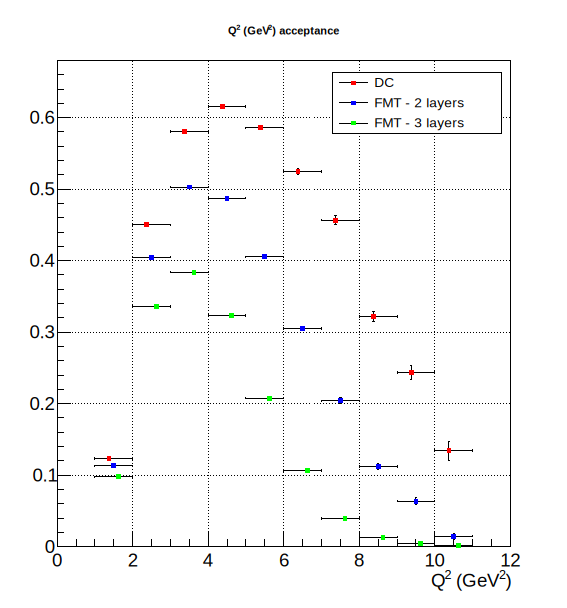
\includegraphics[width=\textwidth]{21q2_acc.pdf}
            \caption{$Q^2$ acceptance.}
            \label{fig::14.21::q2_acc}
        \end{subfigure}
        \hfill
        % nu.
        \begin{subfigure}[b]{0.49\textwidth}
            \centering
            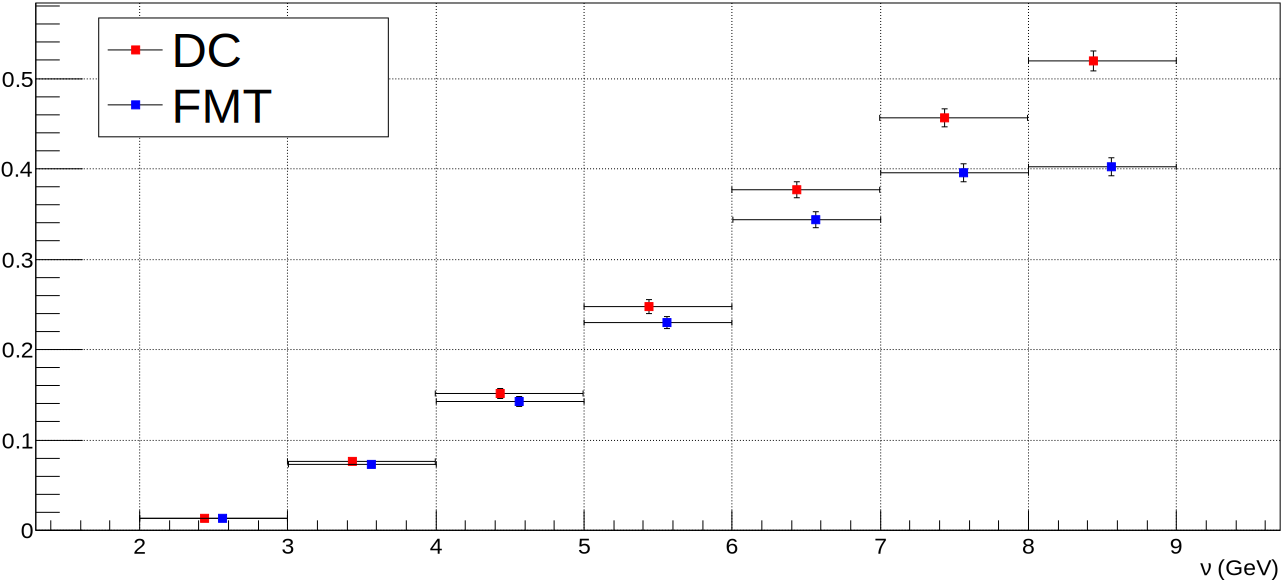
\includegraphics[width=\textwidth]{21nu_acc.pdf}
            \caption{$\nu$ acceptance.}
            \label{fig::14.21::nu_acc}
        \end{subfigure}
        \caption[Electron variables acceptance.]{Electron variables acceptance.
        $\nu$ is integrated in \ref{fig::14.21::q2_acc}, and $Q^2$ is integrated in \ref{fig::14.21::nu_acc}.
        The bin markers are slightly shifted in $x$ to improve legibility.
        Source: Own elaboration, using the \href{https://github.com/bleaktwig/clas12-rge-analysis}{clas12-rge-analysis} software.}
        \label{fig::14.21::electron_acc}
    \end{figure}

    % !TEX root = ../main.tex
\subsubsection{Hadronic Variables}
\label{14.22::hadronic_variables}
    The acceptance of the hadronic variables $z_h$, $p_T^2$, and $\phi_{PQ}$ for $e^-\pi^+$ and $e^-\pi^-$ are presented in Figure \ref{fig::14.22::hadronic_acc}.
    Each one is presented in integrated kinematical region for all electron variables and other hadronic variables.

    % Lower acceptance.
    It's worth noting that these acceptances are lower than those for electron variables.
    This is to be expected, since they require both the trigger electron and at least one hadron to be accepted by the detector.
    This same effect is seen in the $e^-\pi^+$ and $e^-\pi^-$ entries presented in the efficiency Table \ref{tab::14.14::fmt_efficiency_study}.

    % Particle charge-dependent acceptance.
    % TODO. Add phi vs theta (positive particles) plot and explain the difference in acceptances between pi+ and pi- based on that.

    \begin{figure}
        \centering
        % zh pi+.
        \begin{subfigure}[b]{0.49\textwidth}
            \centering
            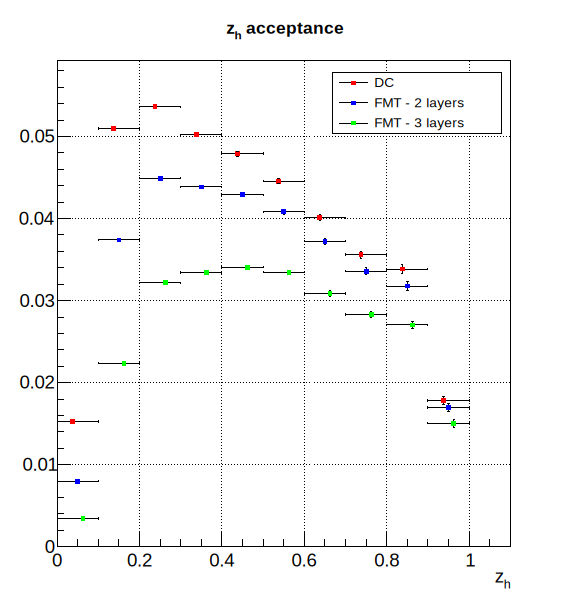
\includegraphics[width=\textwidth]{22zh_acc_211.pdf}
            \caption{$z_h$ acceptance for $e^-\pi^+$.}
            \label{fig::14.22::zh_acc_211}
        \end{subfigure}
        \hfill
        % zh pi-.
        \begin{subfigure}[b]{0.49\textwidth}
            \centering
            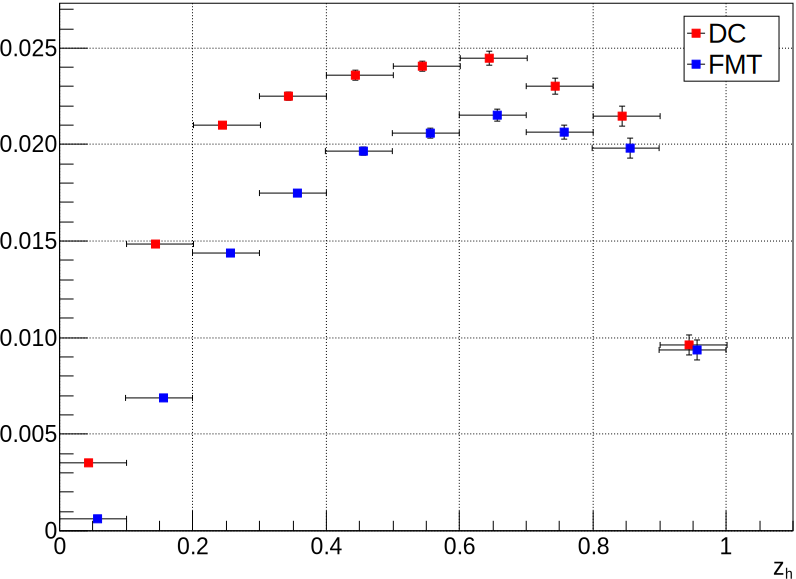
\includegraphics[width=\textwidth]{22zh_acc_-211.pdf}
            \caption{$z_h$ acceptance for $e^-\pi^-$.}
            \label{fig::14.22::zh_acc_-211}
        \end{subfigure}

        \centering
        % pt2 pi+.
        \begin{subfigure}[b]{0.49\textwidth}
            \centering
            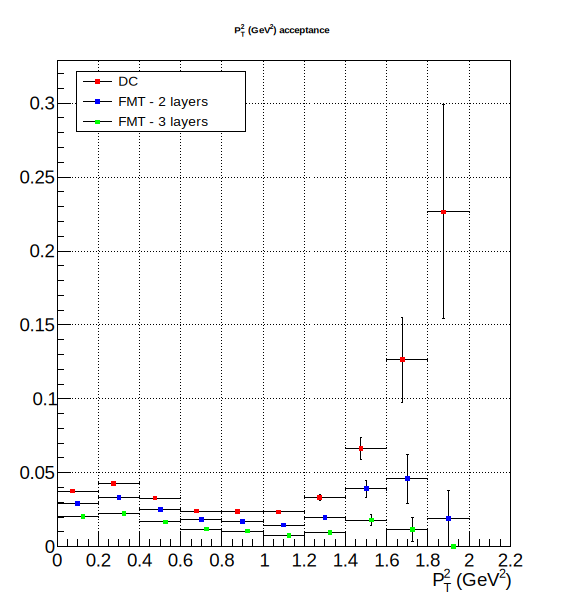
\includegraphics[width=\textwidth]{22pt2_acc_211.pdf}
            \caption{$p_T^2$ acceptance for $e^-\pi^+$.}
            \label{fig::14.22::pt2_acc_211}
        \end{subfigure}
        \hfill
        % pt2 pi-.
        \begin{subfigure}[b]{0.49\textwidth}
            \centering
            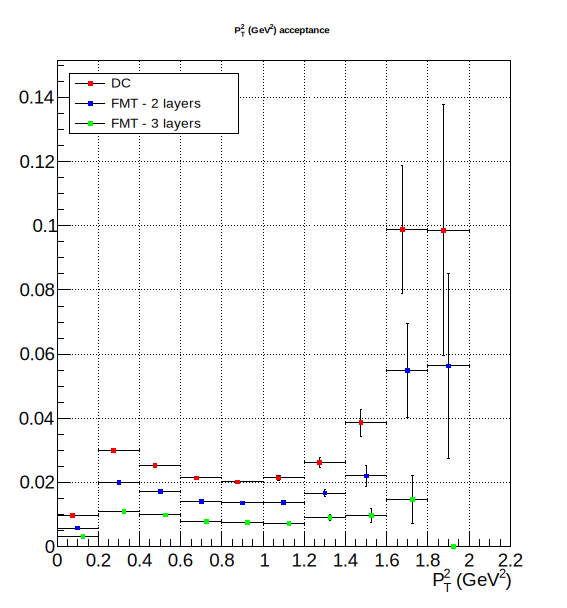
\includegraphics[width=\textwidth]{22pt2_acc_-211.pdf}
            \caption{$p_T^2$ acceptance for $e^-\pi^-$.}
            \label{fig::14.22::pt2_acc_-211}
        \end{subfigure}

        \centering
        % phipq pi+.
        \begin{subfigure}[b]{0.49\textwidth}
            \centering
            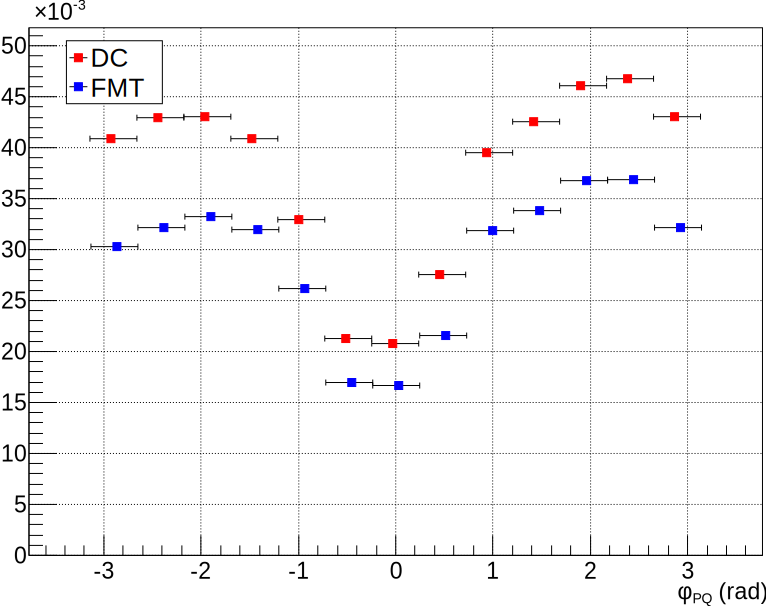
\includegraphics[width=\textwidth]{22phipq_acc_211.pdf}
            \caption{$\phi_{PQ}$ acceptance for $e^-\pi^+$.}
            \label{fig::14.22::phipq_acc_211}
        \end{subfigure}
        \hfill
        % phipq pi-.
        \begin{subfigure}[b]{0.49\textwidth}
            \centering
            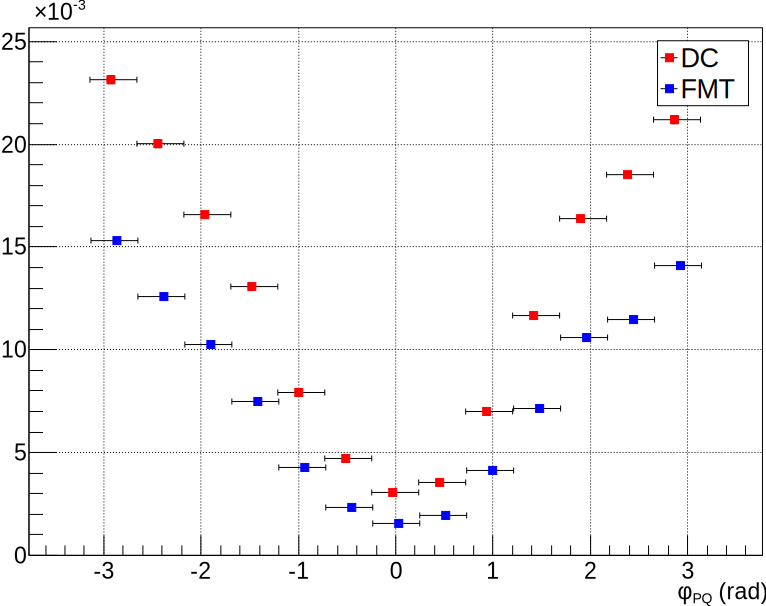
\includegraphics[width=\textwidth]{22phipq_acc_-211.pdf}
            \caption{$\phi_{PQ}$ acceptance for $e^-\pi^-$.}
            \label{fig::14.22::phipq_acc_-211}
        \end{subfigure}
        \caption[hadronic variables acceptance]
        {$z_h$, $p_T^2$, and $\phi_{PQ}$ acceptances for $e^-\pi^+$ and $e^-\pi^-$.
        All electron and other hadronic variables are integrated in all Figures.
        The bin markers are slightly shifted in $x$ to improve legibility.}
        \floatfoot{Source: Own elaboration, using the \href{https://github.com/bleaktwig/clas12-rge-analysis}{clas12-rge-analysis} software.}
        \label{fig::14.22::hadronic_acc}
    \end{figure}


% --+ Plots +-------------------------------------------------------------------
    % \begin{figure}[hbtp]
    %     % Q2.
    %     \begin{subfigure}{.5\textwidth}
    %         \centering
    %         \includegraphics[width=\linewidth]{13dataanalysis/img/40_accbins_q2.pdf}
    %         % \caption{$Q^2$ bins.}
    %         \label{fig::acc_corr_bins_q2}
    %     \end{subfigure}
    %     \begin{subfigure}{.5\textwidth}
    %         \centering
    %         \includegraphics[width=\linewidth]{13dataanalysis/img/40_acccorr_q2.pdf}
    %         % \caption{$Q^2$ acceptance correction results.}
    %         \label{fig::acc_corr_q2}
    %     \end{subfigure}
    %
    %     % nu.
    %     \begin{subfigure}{.5\textwidth}
    %         \centering
    %         \includegraphics[width=\linewidth]{13dataanalysis/img/40_accbins_nu.pdf}
    %         % \caption{$\nu$ bins.}
    %         \label{fig::acc_corr_bins_nu}
    %     \end{subfigure}
    %     \begin{subfigure}{.5\textwidth}
    %         \centering
    %         \includegraphics[width=\linewidth]{13dataanalysis/img/40_acccorr_nu.pdf}
    %         % \caption{$\nu$ acceptance correction results.}
    %         \label{fig::acc_corr_nu}
    %     \end{subfigure}
    %
    %     % zh.
    %     \begin{subfigure}{.5\textwidth}
    %         \centering
    %         \includegraphics[width=\linewidth]{13dataanalysis/img/40_accbins_zh.pdf}
    %         % \caption{$z_h$ bins.}
    %         \label{fig::acc_corr_bins_zh}
    %     \end{subfigure}
    %     \begin{subfigure}{.5\textwidth}
    %         \centering
    %         \includegraphics[width=\linewidth]{13dataanalysis/img/40_acccorr_zh.pdf}
    %         % \caption{$z_h$ acceptance correction results.}
    %         \label{fig::acc_corr_zh}
    %     \end{subfigure}
    %
    %     % PT2.
    %     \begin{subfigure}{.5\textwidth}
    %         \centering
    %         \includegraphics[width=\linewidth]{13dataanalysis/img/40_accbins_pt2.pdf}
    %         % \caption{$P_T^2$ bins.}
    %         \label{fig::acc_corr_bins_pt2}
    %     \end{subfigure}
    %     \begin{subfigure}{.5\textwidth}
    %         \centering
    %         \includegraphics[width=\linewidth]{13dataanalysis/img/40_acccorr_pt2.pdf}
    %         % \caption{$P_T^2$ acceptance correction results.}
    %         \label{fig::acc_corr_pt2}
    %     \end{subfigure}
    %
    %     % phi_PQ.
    %     \begin{subfigure}{.5\textwidth}
    %         \centering
    %         \includegraphics[width=\linewidth]{13dataanalysis/img/40_accbins_phipq.pdf}
    %         % \caption{$\phi_{PQ}$ bins.}
    %         \label{fig::acc_corr_bins_phipq}
    %     \end{subfigure}
    %     \begin{subfigure}{.5\textwidth}
    %         \centering
    %         \includegraphics[width=\linewidth]{13dataanalysis/img/40_acccorr_phipq.pdf}
    %         % \caption{$\phi_{PQ}$ acceptance correction results.}
    %         \label{fig::acc_corr_phipq}
    %     \end{subfigure}
    %
    %     \caption[Acceptance correction results.]{Acceptance correction results for the kinematical variables $Q^2$, $\nu$, $z_h$, $p_T^2$, and $\phi_{PQ}$. On the left plots, the acceptance correction bin edges are shown. On the right, the number of thrown (in red) and simulated (in blue) entries for each of the variables is shown. All other variables are integrated for each plot.}
    %     \label{fig::acc_corr}
    % \end{figure}
